% $Header: /Users/joseph/Documents/LaTeX/beamer/solutions/conference-talks/conference-ornate-20min.en.tex,v 90e850259b8b 2007/01/28 20:48:30 tantau $

\documentclass{beamer}
\usepackage{listings}

% This file is a solution template for:

% - Talk at a conference/colloquium.
% - Talk length is about 20min.
% - Style is ornate.



% Copyright 2004 by Till Tantau <tantau@users.sourceforge.net>.
%
% In principle, this file can be redistributed and/or modified under
% the terms of the GNU Public License, version 2.
%
% However, this file is supposed to be a template to be modified
% for your own needs. For this reason, if you use this file as a
% template and not specifically distribute it as part of a another
% package/program, I grant the extra permission to freely copy and
% modify this file as you see fit and even to delete this copyright
% notice. 


\mode<presentation>
{
  \usetheme{Warsaw}
  % \usetheme{Berkeley}
  % \usecolortheme{crane}
  % \usefonttheme{professionalfonts}
  % or ...

  \setbeamercovered{transparent}
  % or whatever (possibly just delete it)
}


\usepackage[english]{babel}
% or whatever

\usepackage[latin1]{inputenc}
% or whatever

\usepackage{times}
\usepackage[T1]{fontenc}
% Or whatever. Note that the encoding and the font should match. If T1
% does not look nice, try deleting the line with the fontenc.


\title[Fixtures Galore!] % (optional, use only with long paper titles)
{Fixtures Galore!}

\subtitle
{How to Always Have Dummy Data}

\author[digilord] % (optional, use only with lots of authors)
{D. Allen "digilord" Morrigan~\inst{1}}
% - Give the names in the same order as the appear in the paper.
% - Use the \inst{?} command only if the authors have different
%   affiliation.

\institute[Morsby Mechanical] % (optional, but mostly needed)
{
  \inst{1}%
  Morsby Mechanical LLC, Tempe, AZ, USA, North America, Earth, Sol
}
  % \and
  % \inst{2}%
  % Department of Theoretical Philosophy\\
  % University of Elsewhere}
% - Use the \inst command only if there are several affiliations.
% - Keep it simple, no one is interested in your street address.

\date[5 FEB 2015] % (optional, should be abbreviation of conference name)
{Meteor Phoenix}
% - Either use conference name or its abbreviation.
% - Not really informative to the audience, more for people (including
%   yourself) who are reading the slides online

\subject{Fixtures and How to Use Them}
% This is only inserted into the PDF information catalog. Can be left
% out. 



% If you have a file called "university-logo-filename.xxx", where xxx
% is a graphic format that can be processed by latex or pdflatex,
% resp., then you can add a logo as follows:

% \pgfdeclareimage[height=0.5cm]{university-logo}{university-logo-filename}
% \logo{\pgfuseimage{university-logo}}

\pgfdeclareimage[height=0.5cm]{mm-logo}{MM_Logo.png}
\logo{\pgfuseimage{mm-logo}}


% Delete this, if you do not want the table of contents to pop up at
% the beginning of each subsection:
\AtBeginSubsection[]
{
  \begin{frame}<beamer>{Outline}
    \tableofcontents[currentsection,currentsubsection]
  \end{frame}
}


% If you wish to uncover everything in a step-wise fashion, uncomment
% the following command: 

%\beamerdefaultoverlayspecification{<+->}


\begin{document}

\begin{frame}
  \titlepage
\end{frame}

\begin{frame}{Outline}
  \tableofcontents
  % You might wish to add the option [pausesections]
\end{frame}


% Structuring a talk is a difficult task and the following structure
% may not be suitable. Here are some rules that apply for this
% solution: 

% - Exactly two or three sections (other than the summary).
% - At *most* three subsections per section.
% - Talk about 30s to 2min per frame. So there should be between about
%   15 and 30 frames, all told.

% - A conference audience is likely to know very little of what you
%   are going to talk about. So *simplify*!
% - In a 20min talk, getting the main ideas across is hard
%   enough. Leave out details, even if it means being less precise than
%   you think necessary.
% - If you omit details that are vital to the proof/implementation,
%   just say so once. Everybody will be happy with that.

\section{Motivation}

\subsection{Why use fixtures?}

\begin{frame}{Why use fixtures?} %{Creating data is boring.}
  % - A title should summarize the slide in an understandable fashion
  %   for anyone how does not follow everything on the slide itself.

  \begin{itemize}
  \item
    Creating data for your application is boring.
  \item
    Would you rather code or be a data entry monkey?
  \end{itemize}
\end{frame}

\begin{frame}{Reasons to Use Fixtures}

  You can use fixtures for a variety of reasons\dots
  \begin{itemize}
  \pause
  \item visualizing a layout with data
    \begin{itemize}
    \pause
    \item
      how does it look filled in
      \pause
    \item    
      does the styling work with the data being displayed
    \end{itemize}
    \pause
  \item
    trying out different subscription methods
    \begin{itemize}
    \pause
    \item
      do I have too much data?
      \pause
    \item
      is the search I am using efficient?
    \end{itemize}
    \pause
    \item is my schema working for or against my data?
  \item
    And many other possibilities!
    
  \end{itemize}
\end{frame}


\subsection{Fixtures I Commonly Use}

\begin{frame}{Base Users}
\begin{itemize}
  \item We have all done this.
\end{itemize}
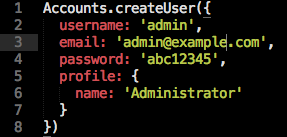
\includegraphics[width=0.5\columnwidth]{admin-fixture.png}

\end{frame}

\begin{frame}{Many Users with Faker}
  \begin{itemize}
    \item generate massive amounts of fake data in the browser and node.js
  \end{itemize}
  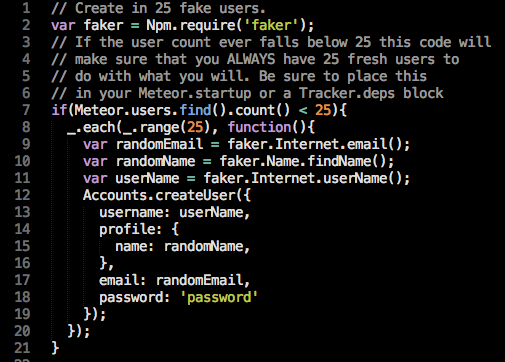
\includegraphics[width=0.5\columnwidth]{many-users.png}
\end{frame}


\section*{Summary}

\begin{frame}{Summary}

  % Keep the summary *very short*.
  \begin{itemize}
  \item
    You should use fixtures to automate data entry of dummy data.
  \item
    Fixtures are your friend. Use them creatively.
  \end{itemize}
  
  % The following outlook is optional.
  \vskip0pt plus.5fill
  \begin{itemize}
  \item
    Outlook
    \begin{itemize}
    \item
      Create a package that adds thousands of fake users.
    \item
      Create a solid search \& pagination package.
    \end{itemize}
  \end{itemize}
\end{frame}

\section*{Your Host}
\begin{frame}{Your Host}
  \begin{block}{DigiLord}
    \begin{itemize}
      \item @digilord (twitter)
      \item digiord@me.com (email \& iMessage)
      \item https://github.com/digilord
      \item IRC in the \#meteor channel as digilord
    \end{itemize}
  \end{block}
\end{frame}


% All of the following is optional and typically not needed. 
\appendix
\section<presentation>*{\appendixname}
\subsection<presentation>*{For Further Reading}

\begin{frame}[allowframebreaks]
  \frametitle<presentation>{For Further Reading}
    
  \begin{thebibliography}{10}
    
  % \beamertemplatebookbibitems
  % Start with overview books.

  % \bibitem{meteor-faker}
  %   A.~Author.
  %   \newblock {\em Handbook of Everything}.
  %   \newblock Some Press, 1990.
 
    
  \beamertemplatearticlebibitems
  % Followed by interesting articles. Keep the list short. 

  \bibitem{digilord}
    meteor-faker
    \newblock Generate massive amounts of fake data.
    \newblock {\em https://github.com/digilord/meteor-faker}, 2014-2015

  \bibitem{marak}
    meteor-faker
    \newblock Generate massive amounts of fake data.
    \newblock {\em https://github.com/Marak/faker.js}, 2013-2015
  \end{thebibliography}
\end{frame}

\end{document}


